%!TEX root = main.tex
\section{Decidability results}

We investigate several decidability and asymptotic complexity issues concerning $k$-synchronizability. In this context, we consider finite-state message passing systems, where each process has a bounded number of local states. First, the reduction of checking $k$-synchronizability to a reachability problem under the synchronous semantics in Section~\ref{sec:verif} demonstrates the decidability of the former. 
Then, we give a class of systems for which the problem of checking whether there exists some $k$ such that they are  $k$-synchronizable is decidable.

\begin{theorem}
The problem of checking $k$-synchronizability of a finite-state system $\mathcal{S}$ is decidable and ???-complete.
\end{theorem}
\begin{proof}
Direct consequence of Theorem~\ref{th:main-verif}.
\end{proof}

\begin{figure}
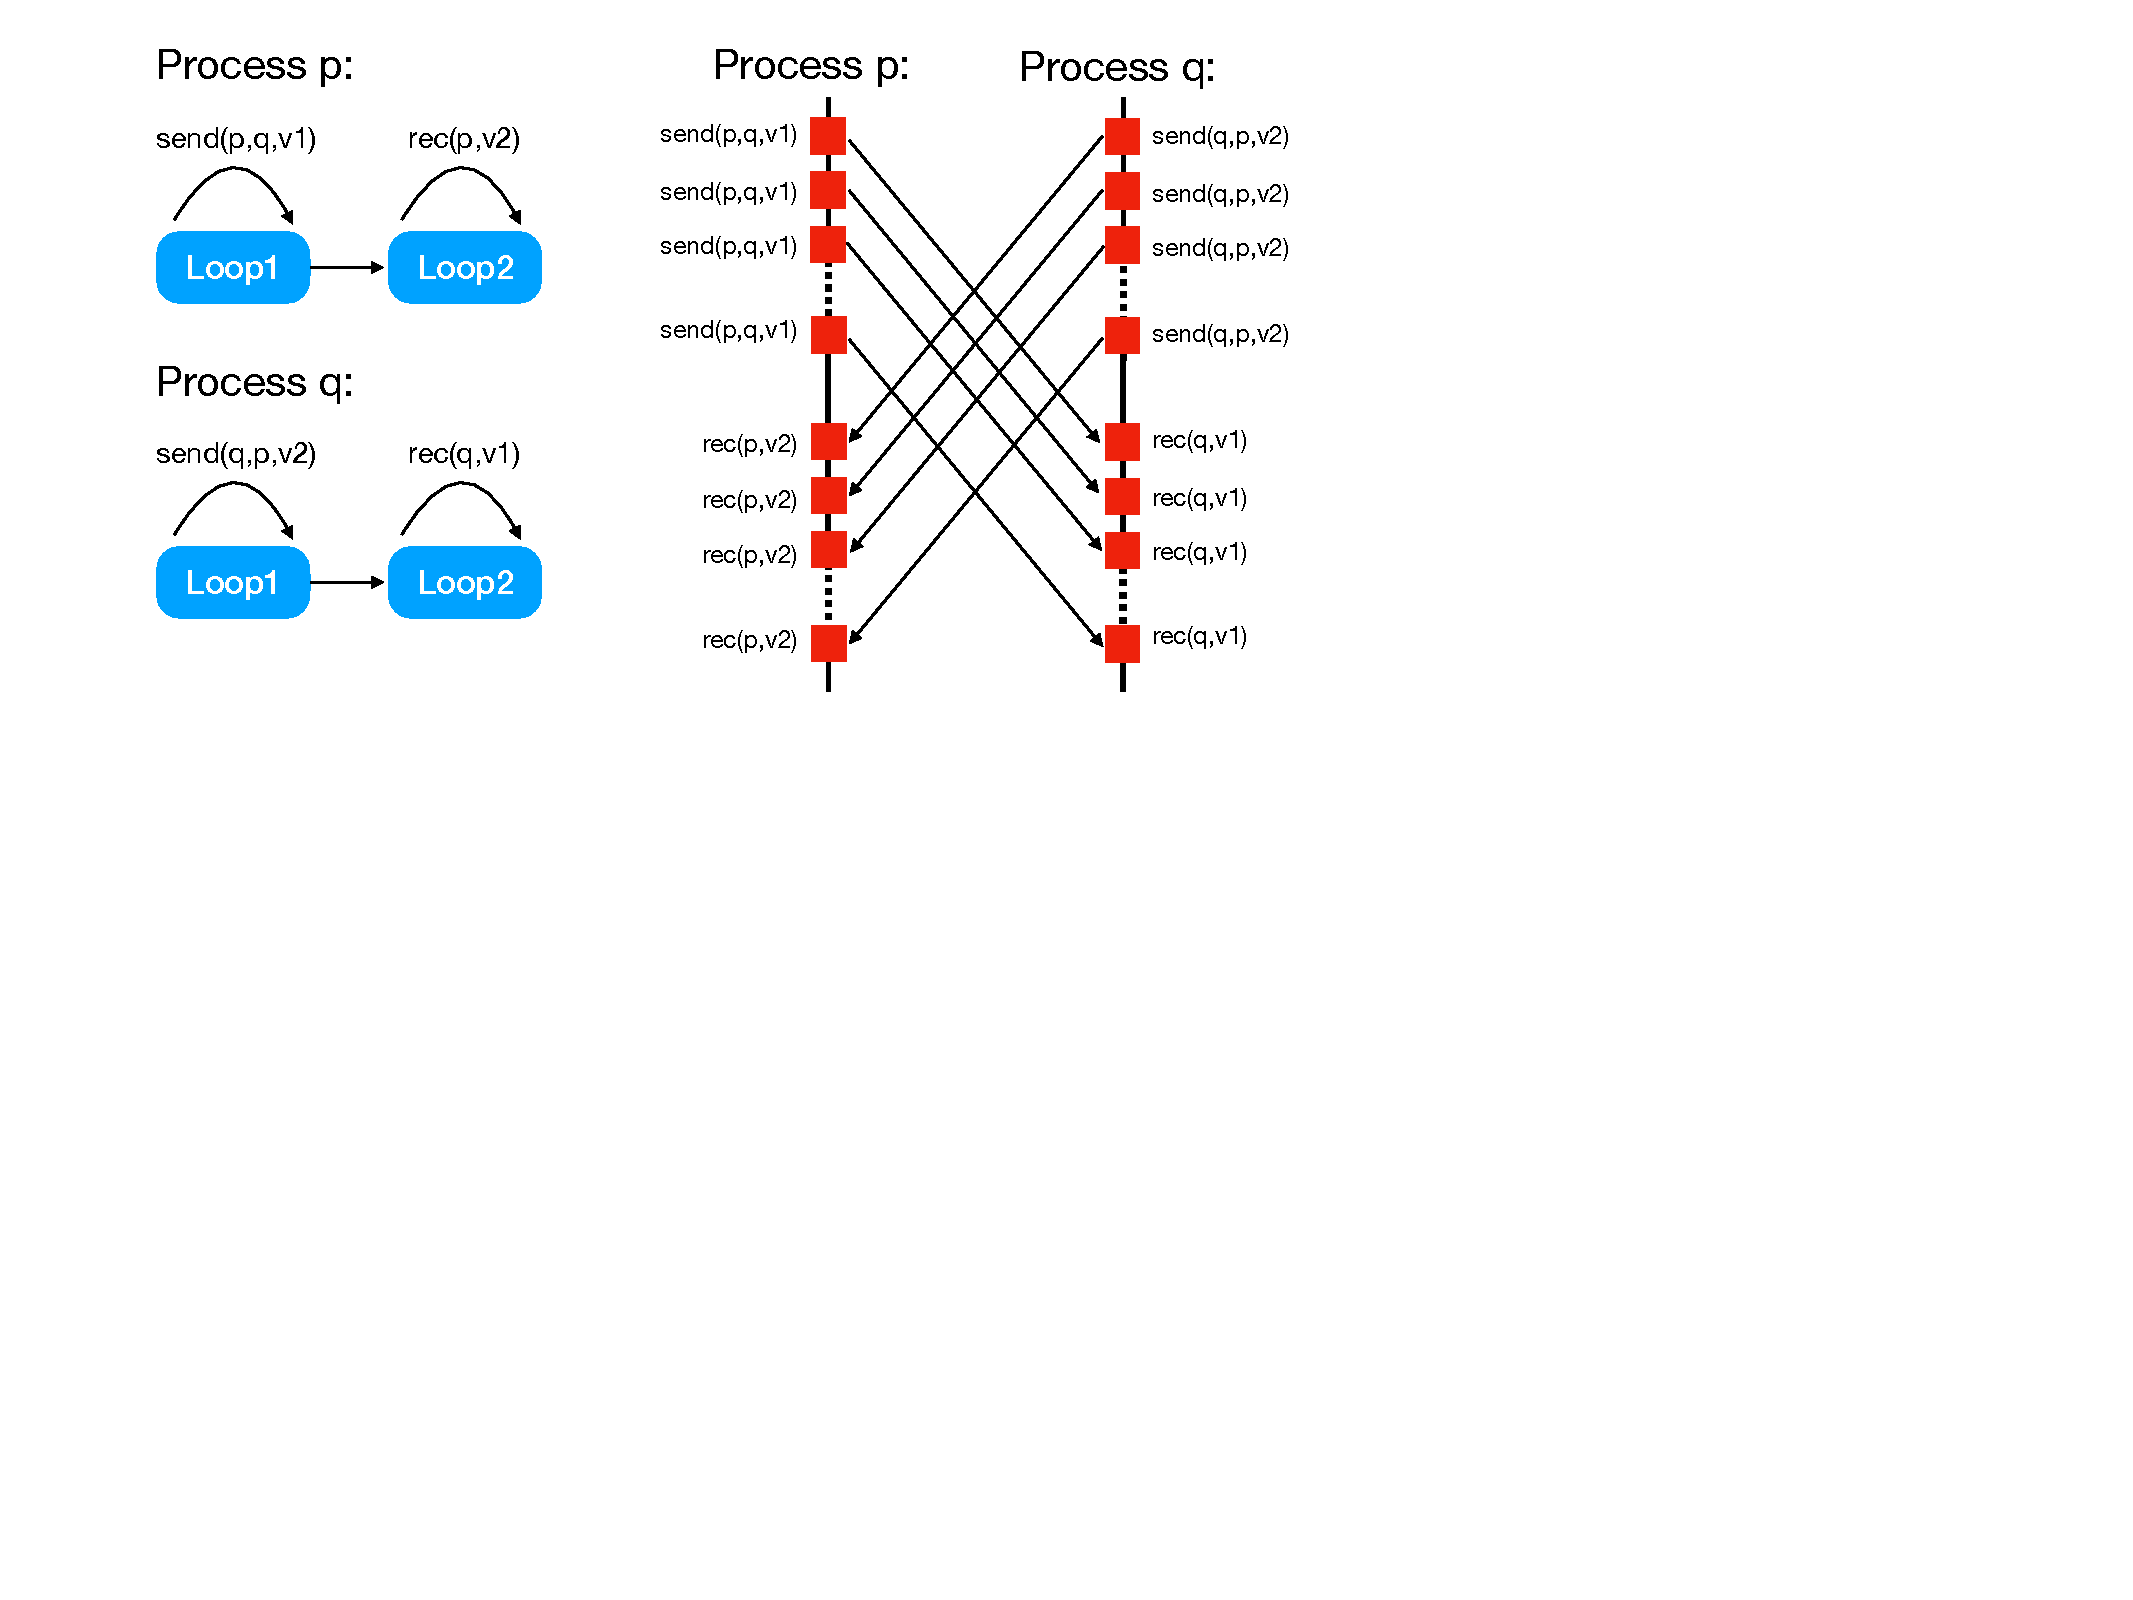
\includegraphics[width=7cm]{Ex-Decidability.pdf}
\caption{An example of a system which is not $k$-synchronizable, for every $k$.}
\label{fig:decid_ex}
\end{figure}

In general, there are two reasons for which a system is not $k$-synchronizable, for every $k$. Either it admits an execution with a bad conflict-graph cycle (e.g., the execution in Figure~\ref{fig:ex-rs-cycle}), or it admits executions with infinitely increasing conflict-graph cycles. Figure~\ref{fig:decid_ex} gives an example of such a system. 
The two loops in each process allow to create executions with unboundedly many send actions before any receive is enabled. However, most of the systems that occur in practice don't 